\documentclass{standalone}
\usepackage{tikz}

\usetikzlibrary{calc}


\begin{document}

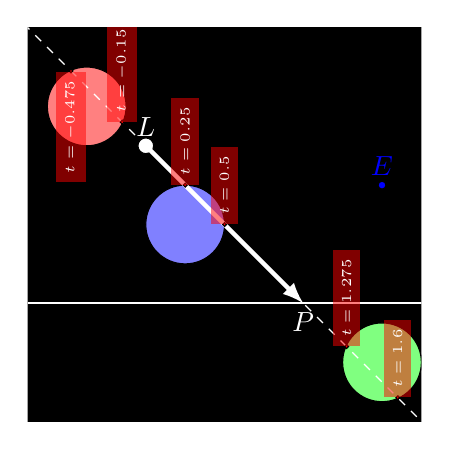
\begin{tikzpicture}[t label/.style={white,rotate=90,right,font=\tiny,fill=red,opacity=0.5,text opacity=1}]
  \path[clip] (-1.5,-1.5) rectangle (3.5,3.5);
  \draw[fill=black,black] (-1.5,-1.5) rectangle (3.5,3.5);
  \draw[thick,white] (-1.5,0) -- (4,0);

  \coordinate (light) at (0,2);
  \coordinate (hit) at (2,0);
  \coordinate (eye) at (3,1.5);
  
  \draw[fill=blue] (eye) circle [radius=0.05cm] node[above,blue] {$E$};
  \draw[fill=white] (light) circle [radius=0.1cm] node [white,above] {$L$};
  \node[anchor=north,white] at (hit) {$P$};

  \coordinate (sphere 1) at (0.5, 1);
  \coordinate (sphere 2) at (-0.75, 2.5);
  \coordinate (sphere 3) at (3, -.75);
  \draw[fill=blue!50] (sphere 1) circle [radius=.5cm];
  \draw[fill=red!50] (sphere 2) circle [radius=.5cm];
  \draw[fill=green!50] (sphere 3) circle [radius=.5cm];

  \draw[white,dashed] ($ (light) ! -1 ! (hit) $) -- ($ (light) ! 2 ! (hit) $);
  \draw[ultra thick,white,-latex] (light) -- (hit);

  \draw[fill=red] ($ (light) ! 0.25 ! (hit) $) circle [radius=0.025cm] node[t label] {$t=0.25$};
  \draw[fill=red] ($ (light) ! 0.5 ! (hit) $) circle [radius=0.025cm] node[t label] {$t=0.5$};
  \draw[fill=red] ($ (light) ! -0.15 ! (hit) $) circle [radius=0.025cm] node[t label] {$t=-0.15$};
  \draw[fill=red] ($ (light) ! -0.475 ! (hit) $) circle [radius=0.025cm] node[t label,left] {$t=-0.475$};
  \draw[fill=red] ($ (light) ! 1.275 ! (hit) $) circle [radius=0.025cm] node[t label] {$t=1.275$};
  \draw[fill=red] ($ (light) ! 1.6 ! (hit) $) circle [radius=0.025cm] node[t label] {$t=1.6$};
\end{tikzpicture}

\end{document}